% Options for packages loaded elsewhere
\PassOptionsToPackage{unicode}{hyperref}
\PassOptionsToPackage{hyphens}{url}
%
\documentclass[
]{article}
\usepackage{amsmath,amssymb}
\usepackage{iftex}
\ifPDFTeX
  \usepackage[T1]{fontenc}
  \usepackage[utf8]{inputenc}
  \usepackage{textcomp} % provide euro and other symbols
\else % if luatex or xetex
  \usepackage{unicode-math} % this also loads fontspec
  \defaultfontfeatures{Scale=MatchLowercase}
  \defaultfontfeatures[\rmfamily]{Ligatures=TeX,Scale=1}
\fi
\usepackage{lmodern}
\ifPDFTeX\else
  % xetex/luatex font selection
\fi
% Use upquote if available, for straight quotes in verbatim environments
\IfFileExists{upquote.sty}{\usepackage{upquote}}{}
\IfFileExists{microtype.sty}{% use microtype if available
  \usepackage[]{microtype}
  \UseMicrotypeSet[protrusion]{basicmath} % disable protrusion for tt fonts
}{}
\makeatletter
\@ifundefined{KOMAClassName}{% if non-KOMA class
  \IfFileExists{parskip.sty}{%
    \usepackage{parskip}
  }{% else
    \setlength{\parindent}{0pt}
    \setlength{\parskip}{6pt plus 2pt minus 1pt}}
}{% if KOMA class
  \KOMAoptions{parskip=half}}
\makeatother
\usepackage{xcolor}
\usepackage[margin=1in]{geometry}
\usepackage{longtable,booktabs,array}
\usepackage{calc} % for calculating minipage widths
% Correct order of tables after \paragraph or \subparagraph
\usepackage{etoolbox}
\makeatletter
\patchcmd\longtable{\par}{\if@noskipsec\mbox{}\fi\par}{}{}
\makeatother
% Allow footnotes in longtable head/foot
\IfFileExists{footnotehyper.sty}{\usepackage{footnotehyper}}{\usepackage{footnote}}
\makesavenoteenv{longtable}
\usepackage{graphicx}
\makeatletter
\def\maxwidth{\ifdim\Gin@nat@width>\linewidth\linewidth\else\Gin@nat@width\fi}
\def\maxheight{\ifdim\Gin@nat@height>\textheight\textheight\else\Gin@nat@height\fi}
\makeatother
% Scale images if necessary, so that they will not overflow the page
% margins by default, and it is still possible to overwrite the defaults
% using explicit options in \includegraphics[width, height, ...]{}
\setkeys{Gin}{width=\maxwidth,height=\maxheight,keepaspectratio}
% Set default figure placement to htbp
\makeatletter
\def\fps@figure{htbp}
\makeatother
\setlength{\emergencystretch}{3em} % prevent overfull lines
\providecommand{\tightlist}{%
  \setlength{\itemsep}{0pt}\setlength{\parskip}{0pt}}
\setcounter{secnumdepth}{5}
\usepackage{booktabs}
\usepackage{longtable}
\usepackage{array}
\usepackage{multirow}
\usepackage{wrapfig}
\usepackage{float}
\usepackage{colortbl}
\usepackage{pdflscape}
\usepackage{tabu}
\usepackage{threeparttable}
\usepackage{threeparttablex}
\usepackage[normalem]{ulem}
\usepackage{makecell}
\usepackage{xcolor}
\usepackage{siunitx}

  \newcolumntype{d}{S[
    input-open-uncertainty=,
    input-close-uncertainty=,
    parse-numbers = false,
    table-align-text-pre=false,
    table-align-text-post=false
  ]}
  
\ifLuaTeX
  \usepackage{selnolig}  % disable illegal ligatures
\fi
\usepackage[]{natbib}
\bibliographystyle{agsm}
\IfFileExists{bookmark.sty}{\usepackage{bookmark}}{\usepackage{hyperref}}
\IfFileExists{xurl.sty}{\usepackage{xurl}}{} % add URL line breaks if available
\urlstyle{same}
\hypersetup{
  pdftitle={Adding Nudge-based Reminders to Monetary Incentives for Promoting Rubella Antibody Testing and Vaccination},
  pdfauthor={Hiroki Kato; Shusaku Sasaki; Fumio Ohtake},
  hidelinks,
  pdfcreator={LaTeX via pandoc}}

\title{Adding Nudge-based Reminders to Monetary Incentives for Promoting Rubella Antibody Testing and Vaccination\thanks{This study is conducted as a part of the Project ``Implementation of EBPM in Japan'\,' undertaken at the Research Institute of Economy, Trade and Industry (RIETI). In completing this paper, we thank participants of the EBPM Study Group and the Discussion Paper Study Group of RIETI for their insightful comments. Prior to conducting a randomized controlled trial on an online survey, this study was approved by the Institutional Review Board of the Graduate School of Economics, Osaka University {[}approval number R020114{]}. Declarations of interest: none. Funding: This research was financially supported by the Ministry of Health, Labour and Welfare, Japan; the Japan Society for the Promotion of Science {[}grant number 20H05632 (F., Ohtake){]}; and Japan Science and Technology Agency {[}grant number JPMJPR21R4 (S., Sasaki){]}.}}
\author{Hiroki Kato \and Shusaku Sasaki \and Fumio Ohtake}
\date{Last updated on September 22, 2023}

\begin{document}
\maketitle
\begin{abstract}
We study effects of combining financial incentives with nudges to promote rubella antibody testing and vaccination. In FY2019, the Japanese government began providing vouchers for free testing and vaccination to men aged 40--57 years. Vouchers were mailed to 40--46-year-old men in FY2019. While those aged 47--57 received vouchers in FY2020, they could obtain vouchers and receive testing and vaccination in FY2019 through applying. Focusing on this policy distinction, we conduct a late-FY2019 online field experiment with Japanese 40--57-year-old men. We randomly send nudge-based reminder messages recommending antibody testing and vaccination, and track self-reported behavior until the end of FY2019. One nudge-based reminder with an altruistic message on fetal harm through infection from men to pregnant women significantly promotes antibody testing and vaccination among those who have already received vouchers as a financial incentive. For those who must apply for vouchers, nudge-based reminders have no promoting effect.
\vskip\baselineskip   
\noindent
\textit{JEL classification}: D90, I12, I18

\noindent
\textit{Keywords}: Rubella; Vaccination; Antibody Test; Text Messages; Reminders; Free Vouchers.
\end{abstract}

\hypertarget{intro}{%
\section{Introduction}\label{intro}}

\hypertarget{background}{%
\section{Background of Rubella Vaccination in Japan}\label{background}}

\hypertarget{experiment}{%
\section{Nationwide Online Survey Experiment}\label{experiment}}

\hypertarget{results}{%
\section{Results}\label{results}}

\hypertarget{sample}{%
\subsection{Study Population}\label{sample}}

Our target population consists of men who did not have antibody testing or vaccinations. We exclude respondents who stated in wave 1 that they had already received either antibody testing or vaccination. In wave 2, we asked respondents whether they had already received either testing or vaccination until wave 1. Thus, when estimating the effect on behavior, we exclude respondents who stated in either wave that they had received either antibody testing or vaccination prior to wave 1.

Our aim is to estimate the effect of text messages in situations where men received monetary incentives as vouchers by default and where they had to incur transaction costs to obtain them. To accomplish this, we create a subsample of men aged 40--46 years and another of men aged 47--56 years. Men in the former subsample automatically received the free vouchers (\emph{default incentive} group). Meanwhile, men in the latter subsample received no incentives or required a costly procedure to get it (\emph{opt-in incentive} group). We believe that most men in the opt-in group did not receive free vouchers in FY2019 because \(77.5\)\% of respondents in wave 1 did not know that rubella routine immunization began in FY2019. Thus, in the default incentive group, monetary incentives and text message reminders are more closely combined than in the opt-in incentive group.

\hypertarget{intention}{%
\subsection{Effect of Text Messages on Intentions}\label{intention}}

This subsection estimates the effect of text messages on intentions. We find that individuals' observable characteristics are balanced across experimental arms in both default incentive and opt-in incentive group (See Table \ref{tab:balance-int-default} and \ref{tab:balance-int-optin} in Appendix). Thus, we first report the difference-in-mean test (t-test) for each group.

\hypertarget{difference-in-mean-test}{%
\subsubsection{Difference-in-mean Test}\label{difference-in-mean-test}}

\begin{figure}
\centering
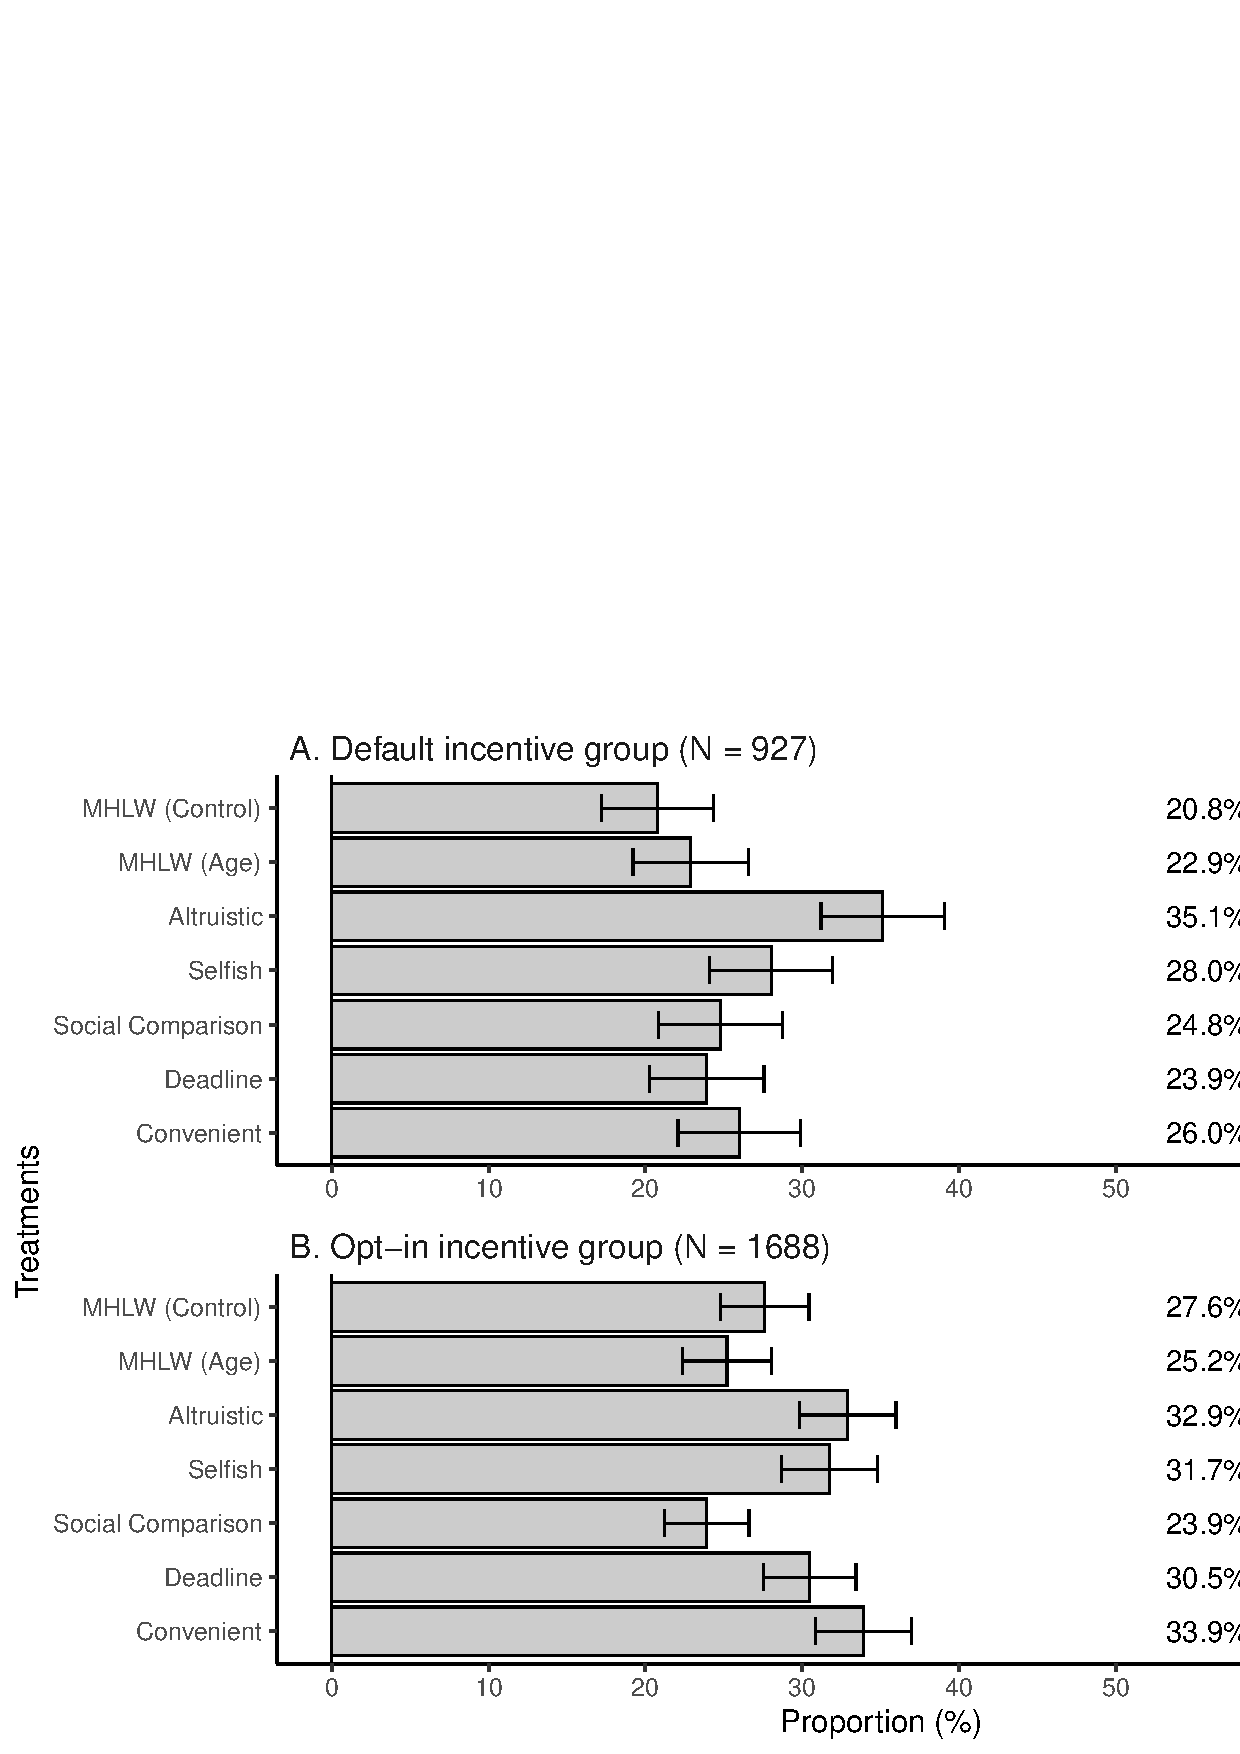
\includegraphics{discussion-paper_files/figure-latex/ttest-int-test-1.pdf}
\caption{\label{fig:ttest-int-test}Effect of Text Messages on Intention for Antibody Testing Notes: Numbers in the figure indicate the proportion of each experimental arm. Error bars indicate the standard error of the mean. Asterisks are p-values of t-tests for the difference-in-mean: * \(p < 0.1\), ** \(p < 0.05\), *** \(p < 0.01\).}
\end{figure}

We show the proportion of intention for antibody testing in each experimental arm for the default incentive group (Panel A) and the opt-in incentive group (Panel B) in Figure \ref{fig:ttest-int-test}. The results show that, in the default incentive group only, the Altruistic message increases the intention for antibody testing by a statistically significant \(14.3\) pp compared to the MHLW (control) message group (\(35.1\)\% in the Altrustic message group versus \(20.8\)\% in the MHLW (control) message group). Because the Altruistic message changes both the age expression and the message content, the effect relative to MHLW (control) can be interpreted as the combined effect of the two changes. However, MHLW (Age), which only changes the age expression, does not increase intention. Thus, the effect of the Altruistic message is attributed to the message content. Compared to MHLW (Age), Altruistic message content increase the intention for antibody testing by \(12.2\) pp (\(35.1\)\% in the Altruistic message group versus \(22.9\)\% in the MHLW (Age) message group), which is statistically significant (see Table \ref{tab:reg-int-woA} in the Appendix).

On the other hand, in the opt-in incentive group, altruistic messages increased intention by \(5.3\) pp, which is statistically insignificant (\(32.9\)\% in the Altrustic message group versus \(27.6\)\% in the MHLW (control) message group).\footnote{However, even in the opt-in incentive group, the Altruistic message content may increase testing intention. Compared to the MHLW(age) message group, the Altruistic messages increased the intention to take the antibody test by \(7.7\) pp (\(32.9\)\% in the Altruistic message group versus \(25.2\)\% in the MHLW (age) message group), which is statistically significant at the 10\% level (see Table \ref{tab:lh-int-woA} in the Appendix).} The regression analysis presented later suggests that the Altruistic message effects may differ between the two incentive groups.

\begin{figure}
\centering
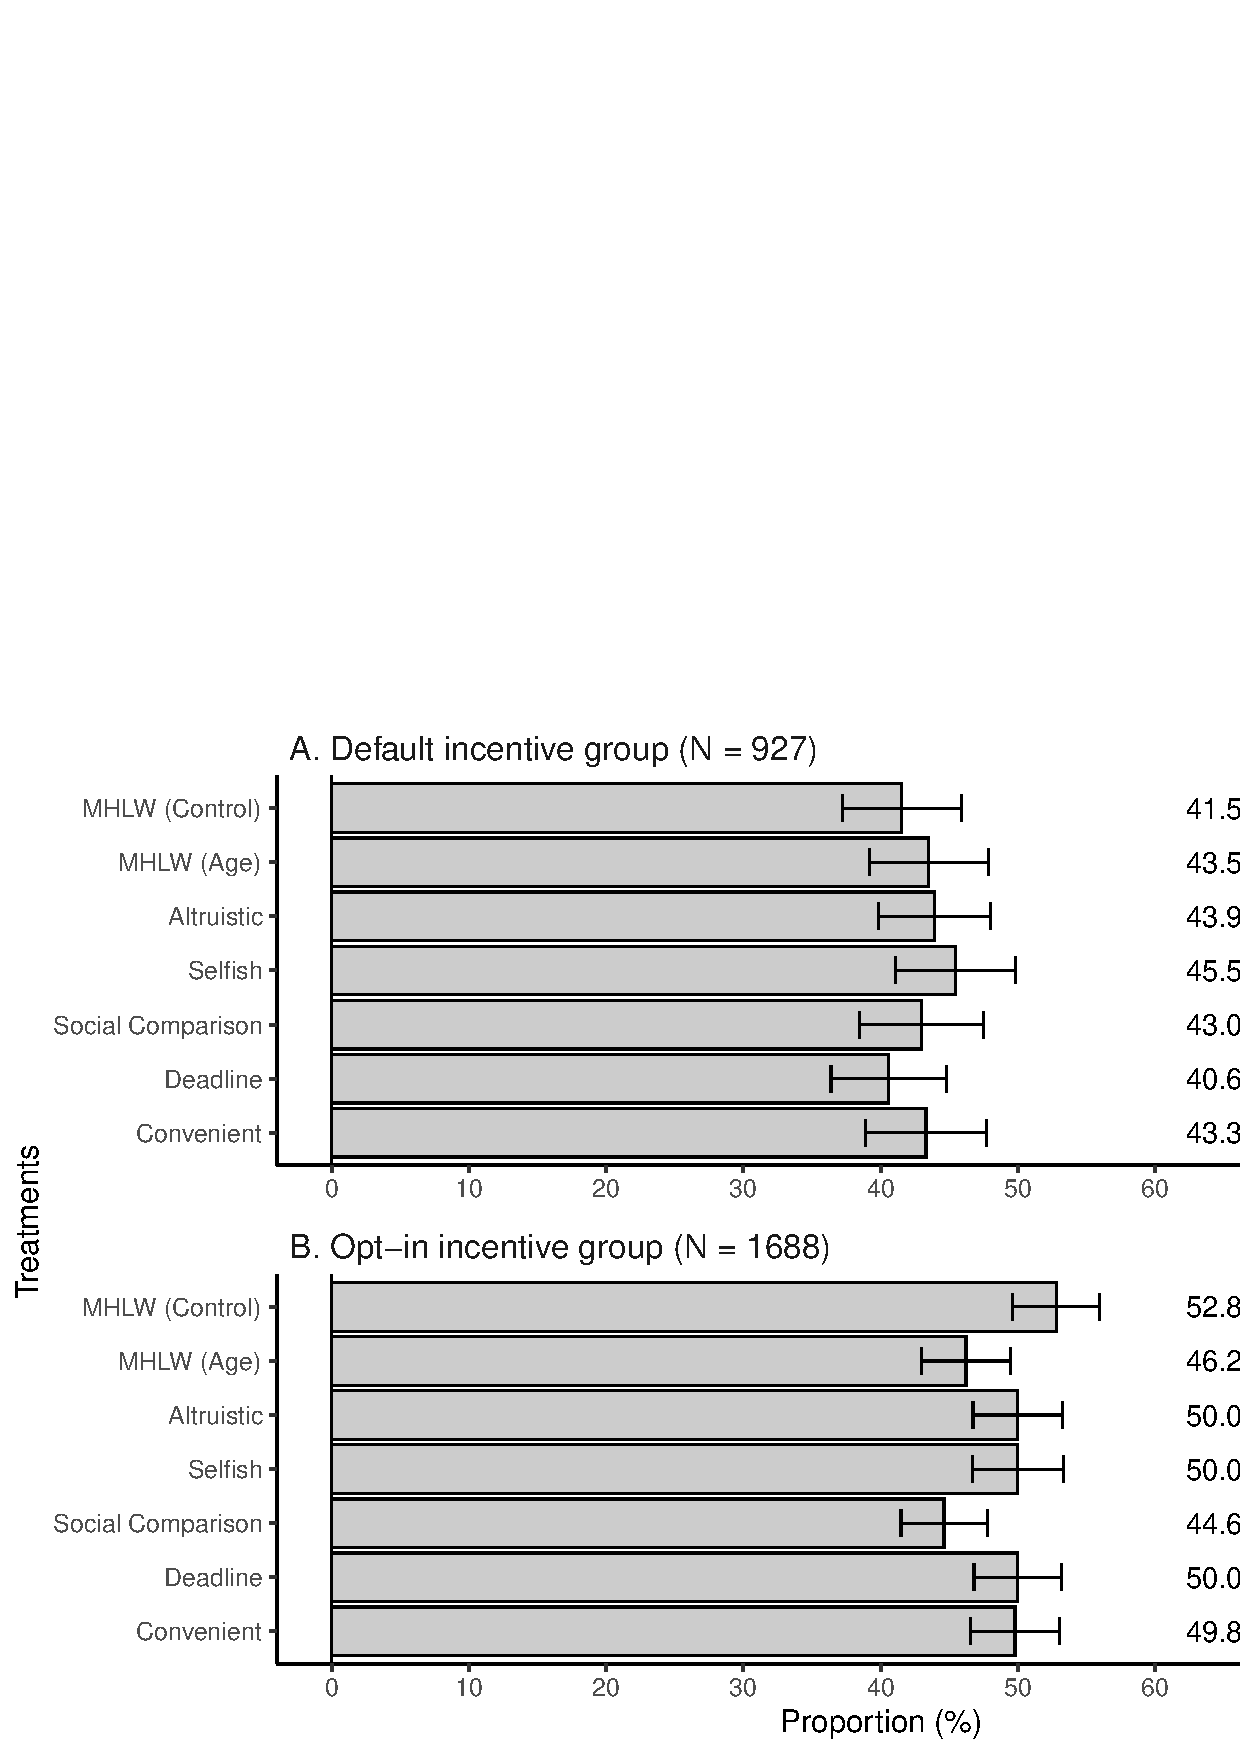
\includegraphics{discussion-paper_files/figure-latex/ttest-int-vacc-1.pdf}
\caption{\label{fig:ttest-int-vacc}Effect of Text Messages on Intention for Vaccination Notes: Numbers in the figure indicate the proportion of each experimental arm. Error bars indicate the standard error of the mean. Asterisks are p-values of t-tests for the difference-in-mean: * \(p < 0.1\), ** \(p < 0.05\), *** \(p < 0.01\).}
\end{figure}

Figure \ref{fig:ttest-int-vacc} depicts the proportions of intention for vaccination for the default incentive group (Panel A) and the opt-in incentive group (Panel B). Results show that in the two incentive groups, most text messages, including the Altruistic messages, do not statistically significantly increase vaccination intentions compared to NHLW (control).

In the opt-in incentive group, the Social Comparison message may lower vaccination intention than the MHLW (control) message (\(44.6\)\% in the Social Comparison message group versus \(52.8\)\% in the MHLW (control) message group). This result is due to the age expression rather than the message content, as social comparison messages hardly lower intention compared to MHLW (age).\footnote{Free-riding may explain why the Social Comparison message content does not increase intention. The Social Comparison message emphasizes that ``one in five people do not have antibodies.'\,' Conversely, four out of five individuals have antibodies. The readers of such a message may have believed that even if they lacked rubella antibodies, the likelihood of infection would be low because 80\% of the population possesses them. When eligible men were required to undergo costly procedures to receive free vouchers, this belief may have made vaccination less beneficial.}

Note that the intention ratio of vaccination in all experimental arms is higher than that of antibody testing in both incentive groups. This result may be explained by the stimulus of the question eliciting the vaccination intention. We asked respondents to report their willingness to vaccinate if they did not have antibodies. This condition may strongly stimulate the need for vaccination. Thus, when assessed by actual behavior, the results may differ.

\hypertarget{regression-analysis}{%
\subsubsection{Regression Analysis}\label{regression-analysis}}

Since age determines whether eligible men received the free vouchers automatically in FY2019, the different effect of text messages for two groups is influenced by the presence or absence of monetary incentives, and by the differences of other dimentions (especially, age) between the two groups. This motivates us to estimate a following linear probability model:
\begin{equation}
\begin{split}
Y_{ij} = &\alpha + \sum_j \beta_j \text{Message}_j + \sum_j \gamma_j (\text{Message}_j \times \text{Opt-in}_i) + \delta \text{Opt-in}_i \\
&+ \lambda X'_{ij} + \epsilon_{ij},
\end{split} \label{eq:regression}
\end{equation}
where \(\text{Message}_j\) is a treatment dummy (the reference group is MHLW (control) message), \(\text{Opt-in}_i\) is a binary variable indicating the opt-in incentive group (47--56 years old), and \(X\) is a set of covariates including age. Our parameter of interest is \(\beta_j\) and \(\gamma_j\). The parameter \(\beta_j\) represents a text message effect for the default incentive group. The linear combination of parameters, \(\beta_j + \gamma_j\), is a text message effect for the opt-in incentive group. The parameter \(\gamma_j\) shows a difference in the message effect between the two groups.

\begin{table}

\caption{\label{tab:reg-int}Regressions of Intention}
\centering
\fontsize{9}{11}\selectfont
\begin{threeparttable}
\begin{tabular}[t]{lcccc}
\toprule
\multicolumn{1}{c}{ } & \multicolumn{2}{c}{Testing} & \multicolumn{2}{c}{Vaccination} \\
\cmidrule(l{3pt}r{3pt}){2-3} \cmidrule(l{3pt}r{3pt}){4-5}
  & (1) & (2) & (3) & (4)\\
\midrule
MHLW (Age) & \num{0.021} & \num{0.039} & \num{0.020} & \num{0.047}\\
 & (\num{0.051}) & (\num{0.049}) & (\num{0.061}) & (\num{0.059})\\
Altruistic & \num{0.144}*** & \num{0.166}*** & \num{0.024} & \num{0.050}\\
 & (\num{0.053}) & (\num{0.049}) & (\num{0.060}) & (\num{0.056})\\
Selfish & \num{0.073} & \num{0.115}** & \num{0.039} & \num{0.087}\\
 & (\num{0.053}) & (\num{0.050}) & (\num{0.061}) & (\num{0.058})\\
Social Comparison & \num{0.040} & \num{0.067} & \num{0.014} & \num{0.039}\\
 & (\num{0.053}) & (\num{0.050}) & (\num{0.063}) & (\num{0.059})\\
Deadline & \num{0.031} & \num{0.039} & \num{-0.010} & \num{0.003}\\
 & (\num{0.051}) & (\num{0.048}) & (\num{0.060}) & (\num{0.058})\\
Convenient & \num{0.052} & \num{0.060} & \num{0.018} & \num{0.032}\\
 & (\num{0.053}) & (\num{0.050}) & (\num{0.062}) & (\num{0.058})\\
Opt-in & \num{0.068} & \num{0.081} & \num{0.113}** & \num{0.077}\\
 & (\num{0.046}) & (\num{0.050}) & (\num{0.054}) & (\num{0.059})\\
MHLW (Age) $\times$ Opt-in & \num{-0.045} & \num{-0.072} & \num{-0.086} & \num{-0.122}*\\
 & (\num{0.065}) & (\num{0.061}) & (\num{0.076}) & (\num{0.072})\\
Altruistic $\times$ Opt-in & \num{-0.091} & \num{-0.121}* & \num{-0.052} & \num{-0.088}\\
 & (\num{0.068}) & (\num{0.064}) & (\num{0.075}) & (\num{0.071})\\
Selfish $\times$ Opt-in & \num{-0.031} & \num{-0.097} & \num{-0.067} & \num{-0.141}*\\
 & (\num{0.068}) & (\num{0.064}) & (\num{0.077}) & (\num{0.073})\\
Social Comparison $\times$ Opt-in & \num{-0.077} & \num{-0.111}* & \num{-0.096} & \num{-0.126}*\\
 & (\num{0.066}) & (\num{0.062}) & (\num{0.077}) & (\num{0.072})\\
Deadline $\times$ Opt-in & \num{-0.003} & \num{-0.006} & \num{-0.018} & \num{-0.024}\\
 & (\num{0.065}) & (\num{0.062}) & (\num{0.075}) & (\num{0.071})\\
Convenient $\times$ Opt-in & \num{0.011} & \num{-0.001} & \num{-0.048} & \num{-0.063}\\
 & (\num{0.067}) & (\num{0.064}) & (\num{0.077}) & (\num{0.072})\\
\midrule
Covariates &  & X &  & X\\
Num.Obs. & \num{2615} & \num{2615} & \num{2615} & \num{2615}\\
R2 & \num{0.009} & \num{0.112} & \num{0.005} & \num{0.118}\\
\bottomrule
\end{tabular}
\begin{tablenotes}
\item Notes: * $p < 0.1$; ** $p < 0.05$; *** $p < 0.01$. Robust standard errors are in parentheses. Covariates are age, education year, annual income, usual health behavior (exercise, medical checkup and ful shot habit) and preference for compliance with social norm.
\end{tablenotes}
\end{threeparttable}
\end{table}

\begin{table}

\caption{\label{tab:lh-int}Text Message Effects for Opt-in Incentive Group Estimated by Regressions}
\centering
\fontsize{9}{11}\selectfont
\begin{threeparttable}
\begin{tabular}[t]{lcccc}
\toprule
\multicolumn{1}{c}{ } & \multicolumn{2}{c}{Testing} & \multicolumn{2}{c}{Vaccination} \\
\cmidrule(l{3pt}r{3pt}){2-3} \cmidrule(l{3pt}r{3pt}){4-5}
  & (1) & (2) & (3) & (4)\\
\midrule
MHLW (Age) & \num{-0.024} & \num{-0.033} & \num{-0.066} & \num{-0.074}*\\
 & (\num{0.040}) & (\num{0.037}) & (\num{0.045}) & (\num{0.042})\\
Altruistic & \num{0.053} & \num{0.045} & \num{-0.028} & \num{-0.038}\\
 & (\num{0.042}) & (\num{0.040}) & (\num{0.046}) & (\num{0.043})\\
Selfish & \num{0.041} & \num{0.017} & \num{-0.028} & \num{-0.054}\\
 & (\num{0.042}) & (\num{0.039}) & (\num{0.046}) & (\num{0.043})\\
Social Comparison & \num{-0.037} & \num{-0.044} & \num{-0.082}* & \num{-0.087}**\\
 & (\num{0.039}) & (\num{0.037}) & (\num{0.045}) & (\num{0.041})\\
Deadline & \num{0.029} & \num{0.033} & \num{-0.028} & \num{-0.021}\\
 & (\num{0.041}) & (\num{0.039}) & (\num{0.045}) & (\num{0.042})\\
Convenient & \num{0.063} & \num{0.059} & \num{-0.030} & \num{-0.031}\\
 & (\num{0.042}) & (\num{0.040}) & (\num{0.045}) & (\num{0.043})\\
Covariates &  & X &  & X\\
\bottomrule
\end{tabular}
\begin{tablenotes}
\item Notes: * $p < 0.1$, ** $p < 0.5$, *** $p < 0.01$. Robust standard errors are in parentheses. Message effects are estimated by a sum of main term of treatment dummy and cross term between treatment dummy and opt-in dummy.
\end{tablenotes}
\end{threeparttable}
\end{table}

The regression analysis also shows that the Altruistic messages increase the intention to take the antibody test only in the default incentive group (Table \ref{tab:reg-int}). Controlling for covariates, altruism messages increase the intention to take the antibody test by \(16.6\) pp in the default incentive group (column (2)). Furthermore, although marginally statistically significant, the effect of this message weakens by \(12.1\) pp as the cost of obtaining a free vaccination ticket becomes more expensive. As a result, the effect of the Altruistic message in the opt-in incentive group is \(4.5\) pp, which is not statistically significant (column (2) in Table \ref{tab:lh-int}). Also statistically insignificant or marginal, the effect of other nudge messages changes in a negative direction as the cost of obtaining free vaccination tickets increases.

Table \ref{tab:reg-int-woA} in the Appendix estimates the effect of modifying the message content, excluding age expression. In the estimation, we exclude from the sample those assigned to MHLW (control). The reference group is MHLW (Age). Controlling for covariates, the Altruistic message content in the default incentive group statistically significantly increased the intention to take the antibody test by \(12.8\) pp, which is the main driver of the positive effect of the Altruistic message in the default incentive group. However, the difference in the effect of message content in the two incentive groups is not statistically significant. Therefore, the F-test results suggest that the Altruistic messages may increase the intention to take the antibody test in the opt-in incentive group (Table \ref{tab:lh-int-woA} in the Appendix).\footnote{An interesting finding is that only in the opt-in incentive group did the content of the Convinient message statistically significantly increase the intention to take the antibody test by about 9 pp.~This group may not have a full understanding of the routine immunization campaign. In fact, the Wave 1 survey shows that only about 20\% of the opt-in incentive group are aware of routine vaccination.}

\hypertarget{behavior}{%
\subsection{Effect of Text Messages on Behavior}\label{behavior}}

This subsection estimates the effect of text messages on behavior. We tested a balance of individual characteristics again because a few respondents dropped out between waves 1 and 2. The results show that the observable characteristics are balanced across experimental arms in both default incentive and opt-in incentive group (see Table \ref{tab:balance-act-default} and \ref{tab:balance-act-optin} in the Appendix). Therefore, we first present the difference-in-mean test (t-test).

\hypertarget{difference-in-mean-test-1}{%
\subsubsection{Difference-in-mean Test}\label{difference-in-mean-test-1}}

\begin{figure}
\centering
\includegraphics{discussion-paper_files/figure-latex/ttest-act-test-1.pdf}
\caption{\label{fig:ttest-act-test}Effect of Text Messages on Behavior for Antibody Testing Notes: Numbers in the figure indicate the proportion of each experimental arm. Error bars indicate the standard error of the mean. Asterisks are p-values of t-tests for the difference-in-mean: * \(p < 0.1\), ** \(p < 0.05\), *** \(p < 0.01\).}
\end{figure}

We show the uptake rate of antibody testing in each experimental arm for the default incentive group (Panel A) and the opt-in incentive group (Panel B) in Figure \ref{fig:ttest-act-test}. We find that, as in the intention case, the Altruistic message statistically significantly increases the antibody test uptake rate compared to the MHLW (control) message by \(7.4\) pp in the default incentive group only (\(10.9\)\% in the Altruistic message group versus \(3.5\)\% in the MHLW (control) message group).

Unlike the intention case, the effect of the Altruistic messages on behavior is not solely due to the content of the message. Compared to MHLW (Age), which only changed the expression of age, the Altruistic message group increases the antibody test uptake rate by \(4.2\) pp (\(10.9\)\% in the Altruistic message group versus \(6.7\)\% in the MHLW (Age) message group). However, regression analysis indicates that this increase is not statistically significant (see Table \ref{tab:reg-act-woA} in the Appendix). Also, although the regression analysis is not statistically significant, modifying the age expression increases the antibody test uptake rate by \(3.2\) pp (\(6.7\)\% in the MHLW (Age) message group versus \(3.5\)\% in the MHLW (Control) message group). Thus, the effect of the Altruistic message on behavior is a combination of the addition of a simple age expression and the revision of the message content.

Selfish messages may boost antibody testing uptake in the default incentive group by \(5.5\) pp (9\% in the Selfish message group versus \(3.5\)\% in the MHLW (control) message group). Moreover, Social Comparison message may also increase antibody testing uptake in the opt-in incentive group (\(4.9\)\% in the Social Comparison message group versus \(3.5\)\% in the MHLW (control) message group). These effects are statistically significant at the 10\% level.

\begin{figure}
\centering
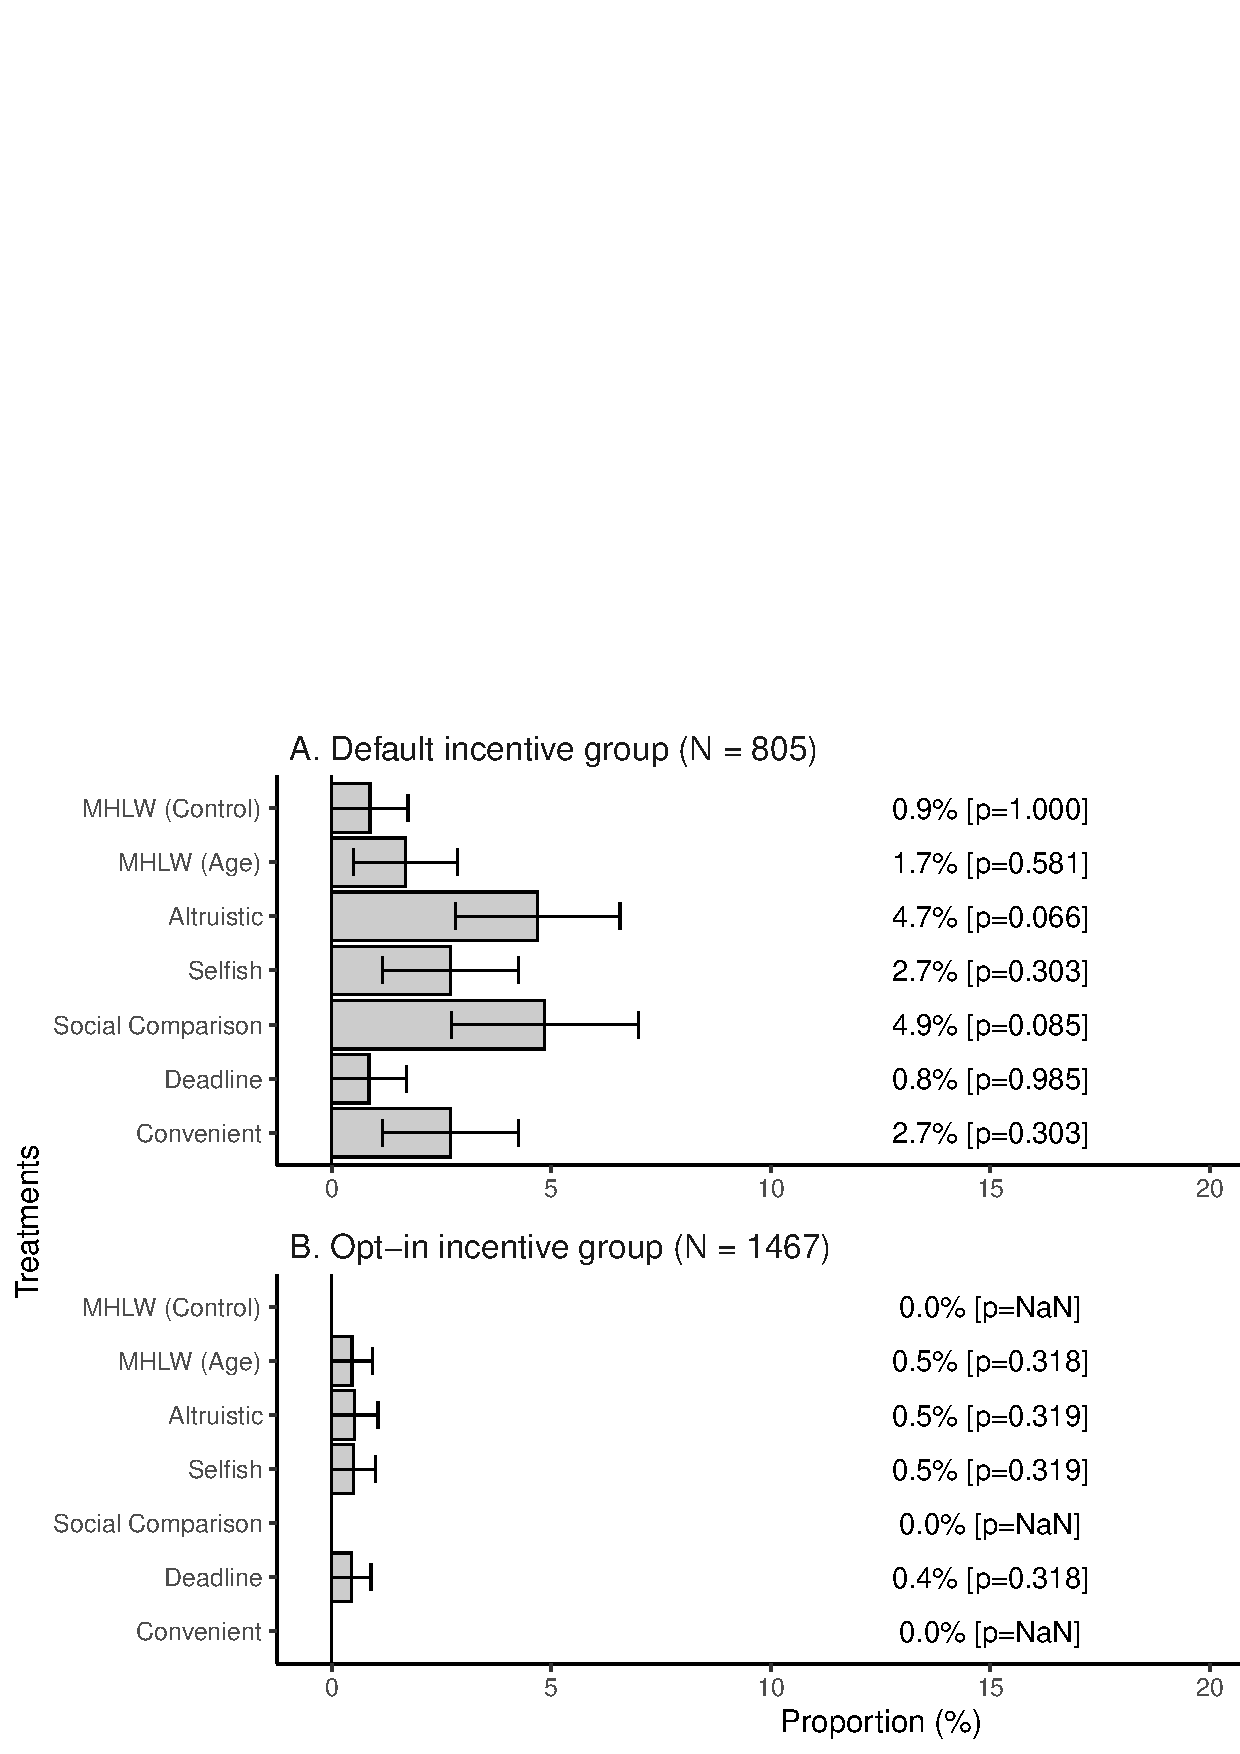
\includegraphics{discussion-paper_files/figure-latex/ttest-act-vacc-1.pdf}
\caption{\label{fig:ttest-act-vacc}Effect of Text Messages on Behavior for Vaccination. Notes: Numbers in the figure indicate the proportion of each experimental arm. Error bars indicate the standard error of the mean. Asterisks are p-values of t-tests for the difference-in-mean: * \(p < 0.1\), ** \(p < 0.05\), *** \(p < 0.01\).}
\end{figure}

Figure \ref{fig:ttest-act-vacc} shows the vaccination rates in each experimental arm for the default incentive group (Panel A) and the opt-in incentive group (Panel B).\footnote{Vaccination is a dummy variable that takes the value of 1 if respondents have been tested and vaccinated. Thus, the vaccination rate can be regarded as the proportion of newly acquired antibodies through vaccination. This outcome variable matches MHLW's policy goal.} In the default incentive group, the Altruistic message may increase the vaccination rate by \(3.8\) pp (\(4.7\)\% in the Altruistic message group versus \(0.9\)\% in the MHLW (control) message group). In the same group, the Social Comparison message may also increase vaccination rate by 4 pp (\(4.9\)\% in the Social Comparison message group versus \(0.9\)\% in the MHLW (control) message group). These effects are statistically siginificant at 10\% level.

\hypertarget{regression-analysis-1}{%
\subsubsection{Regression Analysis}\label{regression-analysis-1}}

\begin{table}

\caption{\label{tab:reg-act}Regressions of Behavior}
\centering
\fontsize{9}{11}\selectfont
\begin{threeparttable}
\begin{tabular}[t]{lcccc}
\toprule
\multicolumn{1}{c}{ } & \multicolumn{2}{c}{Testing} & \multicolumn{2}{c}{Vaccination} \\
\cmidrule(l{3pt}r{3pt}){2-3} \cmidrule(l{3pt}r{3pt}){4-5}
  & (1) & (2) & (3) & (4)\\
\midrule
MHLW (Age) & \num{0.032} & \num{0.029} & \num{0.008} & \num{0.005}\\
 & (\num{0.029}) & (\num{0.028}) & (\num{0.015}) & (\num{0.015})\\
Altruistic & \num{0.075}** & \num{0.073}** & \num{0.038}* & \num{0.037}*\\
 & (\num{0.033}) & (\num{0.032}) & (\num{0.021}) & (\num{0.021})\\
Selfish & \num{0.055}* & \num{0.061}* & \num{0.018} & \num{0.018}\\
 & (\num{0.032}) & (\num{0.032}) & (\num{0.018}) & (\num{0.018})\\
Social Comparison & \num{0.053} & \num{0.056}* & \num{0.040}* & \num{0.040}*\\
 & (\num{0.033}) & (\num{0.033}) & (\num{0.023}) & (\num{0.023})\\
Deadline & \num{0.008} & \num{0.005} & \num{0.000} & \num{-0.002}\\
 & (\num{0.025}) & (\num{0.025}) & (\num{0.012}) & (\num{0.012})\\
Convenient & \num{0.037} & \num{0.038} & \num{0.018} & \num{0.018}\\
 & (\num{0.030}) & (\num{0.030}) & (\num{0.018}) & (\num{0.018})\\
Opt-in & \num{-0.030}* & \num{-0.018} & \num{-0.009} & \num{-0.003}\\
 & (\num{0.018}) & (\num{0.020}) & (\num{0.009}) & (\num{0.012})\\
MHLW (Age) $\times$ Opt-in & \num{-0.028} & \num{-0.026} & \num{-0.003} & \num{-0.002}\\
 & (\num{0.030}) & (\num{0.030}) & (\num{0.015}) & (\num{0.016})\\
Altruistic $\times$ Opt-in & \num{-0.058}* & \num{-0.057}* & \num{-0.033} & \num{-0.032}\\
 & (\num{0.034}) & (\num{0.034}) & (\num{0.021}) & (\num{0.021})\\
Selfish $\times$ Opt-in & \num{-0.045} & \num{-0.054} & \num{-0.013} & \num{-0.013}\\
 & (\num{0.034}) & (\num{0.033}) & (\num{0.018}) & (\num{0.018})\\
Social Comparison $\times$ Opt-in & \num{-0.029} & \num{-0.034} & \num{-0.040}* & \num{-0.039}*\\
 & (\num{0.035}) & (\num{0.035}) & (\num{0.023}) & (\num{0.023})\\
Deadline $\times$ Opt-in & \num{0.001} & \num{0.003} & \num{0.005} & \num{0.006}\\
 & (\num{0.027}) & (\num{0.026}) & (\num{0.013}) & (\num{0.013})\\
Convenient $\times$ Opt-in & \num{-0.032} & \num{-0.031} & \num{-0.018} & \num{-0.018}\\
 & (\num{0.031}) & (\num{0.031}) & (\num{0.018}) & (\num{0.018})\\
\midrule
Covariates &  & X &  & X\\
Num.Obs. & \num{2272} & \num{2272} & \num{2272} & \num{2272}\\
R2 & \num{0.030} & \num{0.047} & \num{0.019} & \num{0.029}\\
\bottomrule
\end{tabular}
\begin{tablenotes}
\item Notes: * $p < 0.1$; ** $p < 0.05$; *** $p < 0.01$. Robust standard errors are in parentheses. Covariates are age, education year, annual income, usual health behavior (exercise, medical checkup and ful shot habit) and preference for compliance with social norm.
\end{tablenotes}
\end{threeparttable}
\end{table}

\begin{table}

\caption{\label{tab:lh-act}Text Message Effects on Behavior for Opt-in Incentive Group Estimated by Regressions}
\centering
\fontsize{9}{11}\selectfont
\begin{threeparttable}
\begin{tabular}[t]{lcccc}
\toprule
\multicolumn{1}{c}{ } & \multicolumn{2}{c}{Testing} & \multicolumn{2}{c}{Vaccination} \\
\cmidrule(l{3pt}r{3pt}){2-3} \cmidrule(l{3pt}r{3pt}){4-5}
  & (1) & (2) & (3) & (4)\\
\midrule
MHLW (Age) & \num{0.005} & \num{0.003} & \num{0.005} & \num{0.004}\\
 & (\num{0.008}) & (\num{0.008}) & (\num{0.005}) & (\num{0.005})\\
Altruistic & \num{0.017} & \num{0.016} & \num{0.005} & \num{0.005}\\
 & (\num{0.011}) & (\num{0.011}) & (\num{0.005}) & (\num{0.005})\\
Selfish & \num{0.010} & \num{0.007} & \num{0.005} & \num{0.005}\\
 & (\num{0.010}) & (\num{0.010}) & (\num{0.005}) & (\num{0.005})\\
Social Comparison & \num{0.023}* & \num{0.022}* & \num{0.000} & \num{0.000}\\
 & (\num{0.012}) & (\num{0.013}) &  & (\num{0.001})\\
Deadline & \num{0.009} & \num{0.009} & \num{0.004} & \num{0.005}\\
 & (\num{0.009}) & (\num{0.009}) & (\num{0.004}) & (\num{0.005})\\
Convenient & \num{0.005} & \num{0.007} & \num{0.000} & \num{0.000}\\
 & (\num{0.008}) & (\num{0.009}) & (\num{0.000}) & (\num{0.001})\\
Covariates &  & X &  & X\\
\bottomrule
\end{tabular}
\begin{tablenotes}
\item  Notes: * $p < 0.1$; ** $p < 0.05$; *** $p < 0.01$. Robust standard errors are in parentheses. Message effects are estimated by a sum of main term of treatment dummy and cross term between treatment dummy and opt-in dummy.
\end{tablenotes}
\end{threeparttable}
\end{table}

As in the case of intention, the different effects of text messages for two incentive group is influenced by dimentions including age difference other than the presence or absence free vouchers. Thus, we estimate a linear probability model (\eqref{eq:regression}) and shows results in Table \ref{tab:reg-act}.

Regression analysis also shows that the Altruistic messages increase antibody test uptake only in the default incentive group. Controlling for covariates, the Altruistic messages increase antibody test uptake by a statistically significant \(7.3\) pp in the default incentive group (column (2)). Furthermore, although the statistical significance is weak, the effect of this message weakens by \(5.7\) pp as the cost of obtaining a free vaccination ticket becomes more expensive. As a result, the effect of the Altruistic message in the opt-in incentive group is \(1.6\) pp, which is not statistically significant (column (2) in Table \ref{tab:lh-act}). A similar trend is observed for the effect on vaccination, but it is weakly statistically significant.

We summarize the results for the other messages. Controlling for covariates, the Selfish message may have increased the antibody test-taking rate in the default incentive group, although the statistical significance is weak (column (2) in Table \ref{tab:reg-act}). We also find that the Social Comparison message may have increased antibody testing rates in the two incentive groups (See column (2) in Table \ref{tab:reg-act} and \ref{tab:lh-act}). However, the effect size is larger in the default incentive group than in the opt-in incentive group (not a statistically significant difference).

As confirmed by the difference-in-means test, the Social Comparison message may increase vaccination rates in the default incentive group (column (4) in Table \ref{tab:reg-act}). Although weakly statistically significant, the effect of this message weakens by \(5.7\) pp as the cost of obtaining vaccination tickets increases. As a result, the Social Comparison message does not increase vaccination rates in the opt-in incentive group (column (4) in Table \ref{tab:lh-act}). Again, the effect of the Altruistic message follows a similar trend.

\hypertarget{monetary-value-of-text-messages}{%
\subsection{Monetary Value of Text Messages}\label{monetary-value-of-text-messages}}

Altruistic (and possibly Social Comparison) messages encourage men who received free vouchers by default to obtain antibody testing and be vaccinated. In this subsection, we attempt to evaluate the effect of these messages in the default incentive group in terms of monetary value. That is, we seek to determine the extent to which the nudge messages increase the monetary value of the rubella vaccination. In other words, we are looking for an amount of additional subsidy equivalent to the message effects in terms of government subsidies.

We use willingness to pay (WTP) for the rubella vaccine.\footnote{Several studies calculate the monetary value of text messages. For example,\cite{Bursztyn2019} calculated it using the two relative effects of financial incentives and text message treatment groups. \cite{Moriwaki2020} also surveyed WTP amounts and calculated monetary value. The latter study is similar to our approach.} Let \(WTP_i\) be an individual's willingness to pay and follow a distribution \(F\). Then, for a given cost \(C\), men will be vaccinated if \(WTP_i \ge C\). The vaccination rate is \(F_0 = 1-F(C)\). Suppose that our treated message changes WTP by \(\beta\). An individual who receives a treated message will be vaccinated if \(WTP_i\ge C-\beta\). The vaccination rate of the treated message group is \(F_1 = 1-F(C-\beta)\). Thus, the treated message effect is \(\tau = F_1-F_0=F(C)-F(C-\beta)\). From the perspective of government subsidies, the amount of subsidy equal to the effect of the nudge message \(\tau\) is \(\beta\). We want to estimate \(\beta\).

Once \(F\), \(C\), and \(\tau\) are determined, we obtain \$\beta \$. To begin, let us discuss the estimation of \(F\) (demand function). We elicit the WTP for vaccination in the first wave before participants read messages. If the vaccination costs 5,000 JPY, we ask respondents if they will get it if the local government pays \(s_j\). The subsidy amounts are \(s_j \in \{0, 1000, 2000, \ldots , 10000\}\). Let \(s_i^{\text{min}}\) be the lowest subsidy at which respondents indicate that they would vaccinate. Let \(s_i^{\text{max}}\) be the highest subsidy that respondents indicate they would not vaccinate. We can identify the willingness to pay for vaccination within the range \([5000 - s_i^{\text{max}}, 5000 - s_i^{\text{min}})\). Thus, without additional assumptions, the demand curve is step-wise, and we estimate the monetary value of the message effect with bounds.\footnote{If respondents indicated that they would not vaccinate at all subsidy amounts, then \(s_i^{\text{max}} = 10000\). However, we cannot define \(s_i^{\text{min}}\) in the data. Therefore, we assume \(s_i^{\text{min}} = 11000\). This assumption does not affect the monetary value of the messages.} To obtain a point estimate, we assume that the true WTP is uniformly distributed within the range \([5000 - s_i^{\text{max}}, 5000 - s_i^{\text{min}})\). Then, The vaccination demand curve can then be linearly interpolated (see Figure \ref{fig:demand-function} in Appendix).

In the default incentive group, eligible males receive free vaccination at no cost. Therefore, the natural setting is \(C=0\). In addition, the message effect \(\tau\) is used for the effect on antibody test uptake. The person taking the antibody test wants to get the antibody, i.e.~the vaccination, against rubella. However, the effect of the message on vaccination is different from the effect on (true) vaccination intention, because people with a positive antibody test result cannot be vaccinated. Therefore, \(\tau\) is not the effect on vaccination, but the effect on antibody testing.

In our framework, \(F_0=1-F(0)\), but one potential concern remains. The message effect \(\tau\) is estimated by the difference from the MHLW (control) group, and \(F(0)\) does not take into account the \(3.5\)\% antibody test uptake rate of the MHLW (control) (see Figure \ref{fig:ttest-act-test}). Assuming that everyone who did not participate in our survey did not take the antibody test after the survey, the uptake rate of MHLW (control) can be considered as an effect of providing the message in the survey. To account for this explicitly, we use \(F_0=(1-F(0))+(F(0)-F(-\alpha))\). The second term is the antibody testing rate of the control group (\(3.5\)\%) under no vaccination cost. The demand function is estimated to be \(F_0=0.7\) and \(\alpha=394\).

\begin{table}

\caption{\label{tab:monetary-value}Estimated Monetary Value of Text Messages}
\centering
\resizebox{\linewidth}{!}{
\fontsize{9}{11}\selectfont
\begin{threeparttable}
\begin{tabular}[t]{lcccccc}
\toprule
\multicolumn{3}{c}{ } & \multicolumn{2}{c}{Monetary value (JPY)} & \multicolumn{2}{c}{Monetary value (USD)} \\
\cmidrule(l{3pt}r{3pt}){4-5} \cmidrule(l{3pt}r{3pt}){6-7}
Text messages & Effect & Baseline + effect & pp & total & pp & total\\
\midrule
MHLW (Age) & 0.032 & 0.732 & 367.854 & 1.946 & 3.679 & 17.690\\
Altruistic & 0.075 & 0.774 & 2037.553 & 10.779 & 20.376 & 97.988\\
Selfish & 0.055 & 0.755 & 744.045 & 3.936 & 7.440 & 35.782\\
Social Comparison & 0.053 & 0.752 & 596.335 & 3.155 & 5.963 & 28.678\\
Deadline & 0.008 & 0.707 & 86.059 & 0.455 & 0.861 & 4.139\\
Convenient & 0.037 & 0.737 & 422.789 & 2.237 & 4.228 & 20.332\\
\bottomrule
\end{tabular}
\begin{tablenotes}
\item We use the effect size of each text messages on antibody testing. Baseline is the sum of the rate of antibody test in the control and the free vaccination rates. The monetary value is the amount per person multiplied by the number of people who received the coupon in 2019 but did not use it until January 2020 ($5.29$ million). We valued it in Japanese Yen and US Dollars (1 USD = 110 JPY). The unit of monetary value per person is 1 JPY and 1 USD, respectively. The unit of total monetary value is 1 billion JPY and 1 million USD, respectively.
\end{tablenotes}
\end{threeparttable}}
\end{table}

We find \(\beta\) holding that \(\tau=F(-\alpha)-F(-\beta)\). Table \ref{tab:monetary-value} shows the estimated message value. The second and third columns show \(\tau\) and \(F_1=\tau+F_0\), respectively. The fourth column shows \(\beta\) in terms of the value of the Japanese yen (in U.S. dollar value, shown in the sixth column). The Altruistic and Social Comparison message, which promotes antibody testing, value about 2,000 JPY (about 18 USD; 40\% of assumed vaccination price) and 600 JPY (about \(5.5\) USD; 12\% of assumed vaccination price), respectively. The total monetary value is the product of the per capita value and the number of people who have not yet used the free vouchers issued in FY2019 (\(5.29\) million as of January 2020). In the fifth column, the Altruistic and Social Comparison messages are worth 10 billion JPY (about 98 million USD) and 3 billion JPY (about 28 million USD), respectively.

\hypertarget{conclusion}{%
\section{Discussion and Conclusions}\label{conclusion}}

This study uses RCTs to investigate effective messages for promoting rubella antibody testing and vaccination in two situations regarding financial incentives. Our experiment reveals that the Altruistic message, which emphasizes the negative externality of infection, increases the intention for antibody testing uptake by \(14.3\) pp among men who already received free vaccination tickets in FY2019. However, this message is less effective for men who incur transaction costs to obtain the vaccination tickets. There may be a statistically significant difference in the effect of this message between the two groups.

Similar results are found for the antibody test uptake. Among men who had already received vaccination vouchers in FY 2019, the Altruistic message increases the antibody test uptake by \(7.5\) pp, which is equivalent to a subsidy of 40\% of the vaccination price. However, this message is less effective for men who incurred the cost of obtaining the vaccination tickets. The effect between the two groups may be statistically significant.

This finding suggests that text message reminders are effective when financial incentives and reminders are closely combined. In addition to the Altruistic message, the Selfish and the Social Comparison message may also raise the intention and the acutual uptake rate for the antibody testing among men who already received the vaccination tickets by default. However, these effect sizes are not large enough to maintain statistical power, requiring a re-examination with a large sample size.

One potential concern is that all behavior-related outcomes were self-reported. These outcomes may contain recall bias. We believe that these biases are less problematic because Wave 2 measures behavior within the last month (the time of Wave 1). The self-reported behavioral outcomes may also be subject to the experimenter demand effect and social desirability bias. To address these biases, our regression analysis directly controls for respondents' psychological factors related to these biases (e.g., following social norm). Even if these biases cannot be eliminated perfectly, they are not fatal to the identification of message effects since this study is a RCT and if these biased exist to the same extent in each group.

Finally, we discuss three points about mechanisms. The first is the mechanism of the Altruistic messages. The effect of Altruistic message (especially on the intention to test for antibodies) is due to a change in the content of the message rather than to the addition of a simple expression of age. The Altruistic message emphasizes the possibility of disability in infants and appeals to the negative externalities of not vaccinating. We analyze the heterogeneity of the message content effect to test which individuals respond more strongly to this message content.

First, in Wave 1, we examine the knowledge that infants born to infected pregnant women may have disabilities and test the heterogeneity of the effect of the altruistic message content on antibody testing intentions depending on whether respondents possessed this knowledge (see column (1) of Table \ref{tab:reg-mechanism} in the Appendix). The results show that the effect of the altruistic message content may be more effective for those who do not possess the knowledge than for those who do. Although there are no statistically significant difference between the effects with and without knowledge, the effects of message content for those with knowledge are not statistically significant. Thus, altruistic message content may modify knowledge about the negative externalities of infection.

It is also important whether a man is altruistic, caring about others' benefit (externality). We investigate whether he feels pleasure in actions for others on a 5 scale in Wave 1 and test the heterogeneous effect of the Altruistic message content by the extent to which he does (see column (2) of Table \ref{tab:reg-mechanism} in the Appendix). The results show that the more altruistic one is, the stronger the effect of the Altruistic message content (this trend is statistically significant). Thus, the Altruistic messages may not be effective for those who do not care about others, even if they perceive negative externalities from reading messages.

The second argument is the effect on vaccination rates. Our experiments reveal that the Altruism and the Social Comparison messages may increase vaccination rates among men who received free vaccination tickets by default. The message effect on vaccination is created through two channels. First, the messages increase the number of negative individuals who need to be vaccinated. Second, the messages encourage unvaccinated negative individuals to vaccinate. Our data suggest that the first channel is more important than the second.

Table \ref{tab:summary-behavior-default} in the Appendix shows the number of men who had antibody testing, who had a negative antibody test, and who were vaccinated in each experimental arm in the default incentive group. This table shows that most of those with negative antibody test results were vaccinated in all experimental arms. Furthermore, the number of negative antibody tests varied between experimental arms. Especially, the 25\% (\(=1/4\)) antibody tests are negative in the MHLW (Control) message group. In contrast, the negative ratios of antibody tests for the Altruistic and Social Comparison messages, which may have a positive effect on vaccination, are 50\% (\(=7/14\)) and 56\% (\(=5/9\)), respectively.\footnote{The negative ratio of antibody testing for the Selfish message, which is only effective for antibody test uptake, is 30\% (\(=3/10\)). This value is similar to the MHLW (control) message.} Thus, the experimental arms with higher vaccination rates have a greater negative ratio, resulting in a positive effect on vaccination. However, the difference in the ratio of negative antibody tests is not statistically significant.

A final discussion is why text messages are ineffective in groups that must incur transaction costs to obtain the free vaccination tickets. Our messages may not increase the value of antibody testing and vaccination sufficiently to outweigh their cost. In addition, another possibility is low awareness of rubella immunization campaign beginning in FY2019. Before presenting the messages, we inquire about the MHLW's policy in Wave 1. As a result, approximately 77.5\% are unaware of the vaccination campaign Thus, even if they read the messages and realized the importance of rubella antibody testing and vaccination, they would believe they had to pay for these preventive actions.\footnote{The fact that many people are unaware of the additional routine rubella vaccinations precludes the possibility that they stopped getting antibody testing and were vaccinated in the first year (FY2019) because they expected to automatically receive the voucher the following year.}

The last two arguments are important issues outside our context. The second argument concerns the targeting of interventions \citep[e.g.,][]{Finkelstein2019}. That is, the question is whether marginal individuals whose behavior is changed by a policy intervention receive significant benefits from that policy. In our context, we suggest that the Altruistic message increases the number of negative individuals who receive a large benefit (vaccination) from the FY2019 vaccination campaign. The third argument relates to testing the effectiveness of vouchers \citep[e.g.,][]{Kacker2022}. The experimental data in this study alone do not allow us to fully explore these arguments, and they are a topic for future research.

\clearpage

\hypertarget{appendix-appendix}{%
\appendix}


\hypertarget{tables-and-figures}{%
\section{Tables and Figures}\label{tables-and-figures}}

\begin{table}[!h]

\caption{\label{tab:covariate-list}List of Covariates}
\centering
\fontsize{9}{11}\selectfont
\begin{tabular}[t]{l>{\raggedright\arraybackslash}p{30em}cc}
\toprule
  & Description & Mean & Std.Dev.\\
\midrule
age & (Wave1) Age as of April 2019 based on year of birth and month of birth. & \num{48.66} & \num{5.69}\\
married & (Wave1) Dummy variable taking one if a respondent is married. & \num{0.58} & \num{0.49}\\
education & (Wave1) Years of education. & \num{14.75} & \num{2.31}\\
income & (Wave1) Household income. For those who did not respond with household income, the overall average was substituted. & \num{684.90} & \num{375.74}\\
noinfo\_income & (Wave1) Dummy variable taking one if a respondent did not answer household income. & \num{0.15} & \num{0.36}\\
exercise\_w1 & (Wave1) Dummy variable taking one if a respondent exercises or plays sports more than once a week. & \num{0.22} & \num{0.42}\\
health\_check & (Wave1) Dummy variable taking one if a respondent has had a medical examination at his/her city or place of employment in the past year from the time of the wave 1. & \num{0.68} & \num{0.46}\\
flushot & (Wave1) Dummy variable taking one if a respondent is vaccinated against influenza every year. & \num{0.27} & \num{0.45}\\
norm & (Wave2) Five-point Likert scale for the question "I wash my hands and gargle frequently during the period from the end of the previous questionnaire response to today." & \num{11.24} & \num{2.32}\\
handwash & (Wave2) Five-point Likert scale for the question "I take my temperature frequently during the period from the end of the previous questionnaire response to today." & \num{3.91} & \num{1.04}\\
temp\_check & (Wave2) Five-point Likert scale for the question "I am refraining from going out during the end of the previous questionnaire response to today." & \num{2.26} & \num{1.22}\\
avoid\_out & (Wave2) Five-point Likert scale for the question "I avoid crowded places when I go out from the end of the previous questionnaire response to today." & \num{2.96} & \num{1.20}\\
avoid\_crowd & (Wave2) Five-point Likert scale for the question "I always wear a medical mask when I go out or meet people during the period from the end of the previous questionnaire response to today." & \num{3.38} & \num{1.10}\\
wear\_mask &  & \num{3.14} & \num{1.38}\\
\bottomrule
\end{tabular}
\end{table}

\begin{table}[!h]

\caption{\label{tab:balance-int-default}Balance Tests for Default Incentive Groups (Sample for Estimating Effect on Intention)}
\centering
\fontsize{9}{11}\selectfont
\begin{threeparttable}
\begin{tabular}[t]{l>{\centering\arraybackslash}p{3em}>{\centering\arraybackslash}p{3em}>{\centering\arraybackslash}p{3em}>{\centering\arraybackslash}p{3em}>{\centering\arraybackslash}p{3em}>{\centering\arraybackslash}p{3em}>{\centering\arraybackslash}p{3em}c}
\toprule
 & MHLW (Control) & MHLW (Age) & Altruistic & Selfish & Social Comparison & Deadline & Convenient & F-test, p-value\\
\midrule
age & 42.862 & 43.046 & 43.135 & 43.045 & 42.909 & 42.906 & 42.866 & 0.874\\
married & 0.408 & 0.458 & 0.412 & 0.417 & 0.455 & 0.478 & 0.480 & 0.785\\
education & 14.654 & 14.473 & 14.595 & 14.205 & 14.099 & 14.348 & 14.575 & 0.446\\
income & 557.562 & 645.556 & 613.156 & 623.542 & 569.530 & 590.422 & 633.487 & 0.149\\
noinfo\_income & 0.162 & 0.168 & 0.203 & 0.197 & 0.157 & 0.130 & 0.181 & 0.706\\
exercise\_w1 & 0.246 & 0.176 & 0.277 & 0.189 & 0.165 & 0.217 & 0.213 & 0.285\\
health\_check & 0.654 & 0.626 & 0.696 & 0.538 & 0.603 & 0.674 & 0.614 & 0.150\\
flushot & 0.238 & 0.260 & 0.203 & 0.144 & 0.140 & 0.239 & 0.236 & 0.055\\
norm & 11.100 & 10.679 & 10.649 & 10.864 & 11.165 & 10.855 & 10.945 & 0.492\\
\bottomrule
\end{tabular}
\begin{tablenotes}
\item Notes: Table \ref{tab:covariate-list} describles variables. Columns 2--8 show sample averages for each experimental arm. Column 9 shows p-value of the joint null hypothesis (F-test).
\end{tablenotes}
\end{threeparttable}
\end{table}

\begin{table}[!h]

\caption{\label{tab:balance-int-optin}Balance Tests for Opt-In Incentive Group (Sample for Estimating Effect on Intention)}
\centering
\fontsize{9}{11}\selectfont
\begin{threeparttable}
\begin{tabular}[t]{l>{\centering\arraybackslash}p{3em}>{\centering\arraybackslash}p{3em}>{\centering\arraybackslash}p{3em}>{\centering\arraybackslash}p{3em}>{\centering\arraybackslash}p{3em}>{\centering\arraybackslash}p{3em}>{\centering\arraybackslash}p{3em}c}
\toprule
 & MHLW (Control) & MHLW (Age) & Altruistic & Selfish & Social Comparison & Deadline & Convenient & F-test, p-value\\
\midrule
age & 51.632 & 51.408 & 51.226 & 51.657 & 51.582 & 51.545 & 51.502 & 0.712\\
married & 0.600 & 0.588 & 0.628 & 0.657 & 0.602 & 0.549 & 0.619 & 0.334\\
education & 14.572 & 14.655 & 14.530 & 14.830 & 14.566 & 14.634 & 14.393 & 0.578\\
income & 712.622 & 707.190 & 687.764 & 677.141 & 656.419 & 707.708 & 710.713 & 0.540\\
noinfo\_income & 0.184 & 0.164 & 0.145 & 0.117 & 0.155 & 0.163 & 0.205 & 0.211\\
exercise\_w1 & 0.156 & 0.193 & 0.239 & 0.230 & 0.183 & 0.203 & 0.218 & 0.252\\
health\_check & 0.632 & 0.664 & 0.701 & 0.683 & 0.653 & 0.659 & 0.644 & 0.742\\
flushot & 0.228 & 0.244 & 0.197 & 0.270 & 0.275 & 0.228 & 0.251 & 0.433\\
norm & 11.336 & 11.340 & 11.346 & 11.304 & 11.187 & 11.122 & 11.293 & 0.922\\
\bottomrule
\end{tabular}
\begin{tablenotes}
\item Notes: Table \ref{tab:covariate-list} describles variables. Columns 2--8 show sample averages for each experimental arm. Column 9 shows p-value of the joint null hypothesis (F-test).
\end{tablenotes}
\end{threeparttable}
\end{table}

\begin{table}

\caption{\label{tab:reg-int-woA}Massage Content Effects on Intentions Compared to MHLW (Age)}
\centering
\fontsize{9}{11}\selectfont
\begin{threeparttable}
\begin{tabular}[t]{lcccc}
\toprule
\multicolumn{1}{c}{ } & \multicolumn{2}{c}{Testing} & \multicolumn{2}{c}{Vaccination} \\
\cmidrule(l{3pt}r{3pt}){2-3} \cmidrule(l{3pt}r{3pt}){4-5}
  & (1) & (2) & (3) & (4)\\
\midrule
Altruistic & \num{0.122}** & \num{0.128}** & \num{0.004} & \num{0.004}\\
 & (\num{0.054}) & (\num{0.051}) & (\num{0.060}) & (\num{0.057})\\
Selfish & \num{0.051} & \num{0.075} & \num{0.019} & \num{0.040}\\
 & (\num{0.054}) & (\num{0.052}) & (\num{0.061}) & (\num{0.059})\\
Social Comparison & \num{0.019} & \num{0.028} & \num{-0.005} & \num{-0.007}\\
 & (\num{0.054}) & (\num{0.052}) & (\num{0.063}) & (\num{0.059})\\
Deadline & \num{0.010} & \num{0.000} & \num{-0.029} & \num{-0.045}\\
 & (\num{0.052}) & (\num{0.050}) & (\num{0.060}) & (\num{0.058})\\
Convenient & \num{0.031} & \num{0.021} & \num{-0.002} & \num{-0.016}\\
 & (\num{0.054}) & (\num{0.051}) & (\num{0.062}) & (\num{0.058})\\
Opt-in & \num{0.023} & \num{0.023} & \num{0.027} & \num{-0.031}\\
 & (\num{0.046}) & (\num{0.052}) & (\num{0.054}) & (\num{0.060})\\
Altruistic $\times$ Opt-in & \num{-0.045} & \num{-0.050} & \num{0.034} & \num{0.032}\\
 & (\num{0.068}) & (\num{0.065}) & (\num{0.075}) & (\num{0.071})\\
Selfish $\times$ Opt-in & \num{0.014} & \num{-0.026} & \num{0.018} & \num{-0.020}\\
 & (\num{0.068}) & (\num{0.065}) & (\num{0.077}) & \vphantom{1} (\num{0.073})\\
Social Comparison $\times$ Opt-in & \num{-0.032} & \num{-0.039} & \num{-0.011} & \num{-0.006}\\
 & (\num{0.067}) & (\num{0.063}) & (\num{0.077}) & (\num{0.073})\\
Deadline $\times$ Opt-in & \num{0.043} & \num{0.065} & \num{0.067} & \num{0.097}\\
 & (\num{0.066}) & (\num{0.063}) & (\num{0.076}) & (\num{0.072})\\
Convenient $\times$ Opt-in & \num{0.056} & \num{0.071} & \num{0.038} & \num{0.059}\\
 & (\num{0.068}) & (\num{0.065}) & (\num{0.077}) & (\num{0.073})\\
\midrule
Covariates &  & X &  & X\\
Num.Obs. & \num{2235} & \num{2235} & \num{2235} & \num{2235}\\
R2 & \num{0.008} & \num{0.108} & \num{0.004} & \num{0.113}\\
\bottomrule
\end{tabular}
\begin{tablenotes}
\item Notes: * $p < 0.1$; ** $p < 0.05$; *** $p < 0.01$. Robust standard errors are in parentheses. We exclude from the sample those assigned to MHLW (control). The reference group is MHLW (Age). Covariates are age, education year, annual income, usual health behavior (exercise, medical checkup and ful shot habit) and preference for compliance with social norm.
\end{tablenotes}
\end{threeparttable}
\end{table}

\begin{table}

\caption{\label{tab:lh-int-woA}Message Content Effects for Opt-in Incentive Group Estimated by Regressions}
\centering
\fontsize{9}{11}\selectfont
\begin{threeparttable}
\begin{tabular}[t]{lcccc}
\toprule
\multicolumn{1}{c}{ } & \multicolumn{2}{c}{Testing} & \multicolumn{2}{c}{Vaccination} \\
\cmidrule(l{3pt}r{3pt}){2-3} \cmidrule(l{3pt}r{3pt}){4-5}
  & (1) & (2) & (3) & (4)\\
\midrule
Altruistic & \num{0.077}* & \num{0.077}* & \num{0.038} & \num{0.036}\\
 & (\num{0.042}) & (\num{0.040}) & (\num{0.046}) & (\num{0.043})\\
Selfish & \num{0.065} & \num{0.049} & \num{0.038} & \num{0.020}\\
 & (\num{0.042}) & (\num{0.039}) & (\num{0.046}) & (\num{0.044})\\
Social Comparison & \num{-0.013} & \num{-0.011} & \num{-0.016} & \num{-0.013}\\
 & (\num{0.039}) & (\num{0.036}) & (\num{0.045}) & (\num{0.042})\\
Deadline & \num{0.053} & \num{0.065}* & \num{0.038} & \num{0.053}\\
 & (\num{0.041}) & (\num{0.039}) & (\num{0.046}) & (\num{0.043})\\
Convenient & \num{0.087}** & \num{0.092}** & \num{0.036} & \num{0.043}\\
 & (\num{0.042}) & (\num{0.039}) & (\num{0.046}) & (\num{0.043})\\
Covariates &  & X &  & X\\
\bottomrule
\end{tabular}
\begin{tablenotes}
\item Notes: * $p < 0.1$; ** $p < 0.05$; *** $p < 0.01$. Robust standard errors are in parentheses. We exclude from the sample those assigned to MHLW (control). The reference group is MHLW (Age). Message effects are estimated by a sum of main term of treatment dummy and cross term between treatment dummy and opt-in dummy.
\end{tablenotes}
\end{threeparttable}
\end{table}

\begin{table}[!h]

\caption{\label{tab:balance-act-default}Balance Tests for Default Incentive Group (Sample for Estimating Effect on Behavior)}
\centering
\fontsize{9}{11}\selectfont
\begin{threeparttable}
\begin{tabular}[t]{l>{\centering\arraybackslash}p{3em}>{\centering\arraybackslash}p{3em}>{\centering\arraybackslash}p{3em}>{\centering\arraybackslash}p{3em}>{\centering\arraybackslash}p{3em}>{\centering\arraybackslash}p{3em}>{\centering\arraybackslash}p{3em}c}
\toprule
 & MHLW (Control) & MHLW (Age) & Altruistic & Selfish & Social Comparison & Deadline & Convenient & F-test, p-value\\
\midrule
age & 42.861 & 43.059 & 43.102 & 43.036 & 42.893 & 42.898 & 42.964 & 0.953\\
married & 0.391 & 0.454 & 0.391 & 0.360 & 0.437 & 0.466 & 0.477 & 0.467\\
education & 14.496 & 14.471 & 14.547 & 14.126 & 14.010 & 14.407 & 14.595 & 0.474\\
income & 548.244 & 649.778 & 614.512 & 599.124 & 555.083 & 591.597 & 637.056 & 0.102\\
noinfo\_income & 0.174 & 0.126 & 0.203 & 0.207 & 0.146 & 0.136 & 0.171 & 0.522\\
exercise\_w1 & 0.252 & 0.185 & 0.266 & 0.171 & 0.165 & 0.195 & 0.225 & 0.375\\
health\_check & 0.643 & 0.639 & 0.680 & 0.532 & 0.631 & 0.661 & 0.640 & 0.391\\
flushot & 0.235 & 0.261 & 0.227 & 0.135 & 0.146 & 0.246 & 0.207 & 0.082\\
norm & 11.174 & 10.706 & 10.758 & 11.063 & 11.204 & 10.831 & 10.982 & 0.523\\
handwash & 3.861 & 3.916 & 3.797 & 3.757 & 3.767 & 3.915 & 3.829 & 0.835\\
temp\_check & 2.139 & 2.235 & 2.414 & 2.126 & 2.204 & 2.203 & 2.117 & 0.535\\
avoid\_out & 3.096 & 3.034 & 3.047 & 2.793 & 2.932 & 3.025 & 2.928 & 0.544\\
avoid\_crowd & 3.296 & 3.336 & 3.273 & 3.234 & 3.350 & 3.305 & 3.324 & 0.990\\
wear\_mask & 2.930 & 3.076 & 3.109 & 3.009 & 3.010 & 3.144 & 3.207 & 0.794\\
\bottomrule
\end{tabular}
\begin{tablenotes}
\item Notes: Table \ref{tab:covariate-list} describles variables. Columns 2--8 show sample averages for each experimental arm. Column 9 shows p-value of the joint null hypothesis (F-test).
\end{tablenotes}
\end{threeparttable}
\end{table}

\begin{table}[!h]

\caption{\label{tab:balance-act-optin}Balance Tests for Opt-in Incentive Group (Sample for Estimating Effect on Behavior)}
\centering
\fontsize{9}{11}\selectfont
\begin{threeparttable}
\begin{tabular}[t]{l>{\centering\arraybackslash}p{3em}>{\centering\arraybackslash}p{3em}>{\centering\arraybackslash}p{3em}>{\centering\arraybackslash}p{3em}>{\centering\arraybackslash}p{3em}>{\centering\arraybackslash}p{3em}>{\centering\arraybackslash}p{3em}c}
\toprule
 & MHLW (Control) & MHLW (Age) & Altruistic & Selfish & Social Comparison & Deadline & Convenient & F-test, p-value\\
\midrule
age & 51.695 & 51.394 & 51.179 & 51.662 & 51.421 & 51.605 & 51.512 & 0.564\\
married & 0.591 & 0.560 & 0.611 & 0.652 & 0.598 & 0.547 & 0.596 & 0.407\\
education & 14.505 & 14.620 & 14.553 & 14.876 & 14.593 & 14.610 & 14.345 & 0.472\\
income & 712.165 & 707.809 & 686.355 & 671.407 & 644.798 & 699.289 & 718.575 & 0.370\\
noinfo\_income & 0.173 & 0.157 & 0.137 & 0.114 & 0.159 & 0.166 & 0.222 & 0.142\\
exercise\_w1 & 0.159 & 0.194 & 0.232 & 0.229 & 0.173 & 0.211 & 0.202 & 0.432\\
health\_check & 0.632 & 0.667 & 0.684 & 0.677 & 0.645 & 0.673 & 0.631 & 0.849\\
flushot & 0.223 & 0.245 & 0.189 & 0.264 & 0.280 & 0.215 & 0.241 & 0.376\\
norm & 11.355 & 11.329 & 11.384 & 11.189 & 11.220 & 11.224 & 11.222 & 0.964\\
handwash & 3.823 & 3.889 & 3.926 & 3.751 & 3.836 & 3.861 & 3.867 & 0.769\\
temp\_check & 2.095 & 2.204 & 2.221 & 2.100 & 2.136 & 2.085 & 2.182 & 0.841\\
avoid\_out & 2.886 & 2.889 & 2.932 & 2.866 & 2.855 & 2.964 & 2.941 & 0.960\\
avoid\_crowd & 3.295 & 3.361 & 3.447 & 3.239 & 3.313 & 3.309 & 3.433 & 0.437\\
wear\_mask & 3.082 & 3.176 & 3.116 & 3.144 & 2.977 & 2.942 & 3.010 & 0.533\\
\bottomrule
\end{tabular}
\begin{tablenotes}
\item Notes: Table \ref{tab:covariate-list} describles variables. Columns 2--8 show sample averages for each experimental arm. Column 9 shows p-value of the joint null hypothesis (F-test).
\end{tablenotes}
\end{threeparttable}
\end{table}

\begin{table}

\caption{\label{tab:reg-act-woA}Message Content Effects on Behaivor Compared to MHLW (Age)}
\centering
\fontsize{9}{11}\selectfont
\begin{threeparttable}
\begin{tabular}[t]{lcccc}
\toprule
\multicolumn{1}{c}{ } & \multicolumn{2}{c}{Testing} & \multicolumn{2}{c}{Vaccination} \\
\cmidrule(l{3pt}r{3pt}){2-3} \cmidrule(l{3pt}r{3pt}){4-5}
  & (1) & (2) & (3) & (4)\\
\midrule
Altruistic & \num{0.042} & \num{0.045} & \num{0.030} & \num{0.032}\\
 & (\num{0.036}) & (\num{0.036}) & (\num{0.022}) & (\num{0.022})\\
Selfish & \num{0.023} & \num{0.032} & \num{0.010} & \num{0.013}\\
 & (\num{0.036}) & (\num{0.035}) & (\num{0.019}) & (\num{0.020})\\
Social Comparison & \num{0.020} & \num{0.027} & \num{0.032} & \num{0.034}\\
 & (\num{0.036}) & (\num{0.036}) & (\num{0.024}) & (\num{0.025})\\
Deadline & \num{-0.025} & \num{-0.024} & \num{-0.008} & \num{-0.007}\\
 & (\num{0.030}) & (\num{0.029}) & (\num{0.015}) & (\num{0.014})\\
Convenient & \num{0.005} & \num{0.009} & \num{0.010} & \num{0.013}\\
 & (\num{0.034}) & (\num{0.034}) & (\num{0.019}) & (\num{0.019})\\
Opt-in & \num{-0.058}** & \num{-0.046}* & \num{-0.012} & \num{-0.002}\\
 & (\num{0.024}) & (\num{0.026}) & (\num{0.013}) & (\num{0.015})\\
Altruistic $\times$ Opt-in & \num{-0.030} & \num{-0.031} & \num{-0.029} & \num{-0.031}\\
 & (\num{0.038}) & (\num{0.038}) & (\num{0.023}) & (\num{0.024})\\
Selfish $\times$ Opt-in & \num{-0.017} & \num{-0.027} & \num{-0.010} & \num{-0.012}\\
 & (\num{0.037}) & (\num{0.037}) & (\num{0.021}) & (\num{0.021})\\
Social Comparison $\times$ Opt-in & \num{-0.001} & \num{-0.008} & \num{-0.036} & \num{-0.038}\\
 & (\num{0.038}) & (\num{0.039}) & (\num{0.025}) & (\num{0.025})\\
Deadline $\times$ Opt-in & \num{0.029} & \num{0.030} & \num{0.008} & \num{0.008}\\
 & (\num{0.031}) & (\num{0.031}) & (\num{0.016}) & (\num{0.016})\\
Convenient $\times$ Opt-in & \num{-0.004} & \num{-0.004} & \num{-0.015} & \num{-0.017}\\
 & (\num{0.035}) & (\num{0.035}) & (\num{0.020}) & (\num{0.020})\\
\midrule
Covariates &  & X &  & X\\
Num.Obs. & \num{1937} & \num{1937} & \num{1937} & \num{1937}\\
R2 & \num{0.029} & \num{0.047} & \num{0.019} & \num{0.030}\\
\bottomrule
\end{tabular}
\begin{tablenotes}
\item Notes: * $p < 0.1$; ** $p < 0.05$; *** $p < 0.01$. Robust standard errors are in parentheses. We exclude from the sample those assigned to MHLW (control). The reference group is MHLW (Age). Covariates are age, education year, annual income, usual health behavior (exercise, medical checkup and ful shot habit) and preference for compliance with social norm.
\end{tablenotes}
\end{threeparttable}
\end{table}

\begin{table}

\caption{\label{tab:lh-act-woA}Message Content Effects for Opt-in Incentive Group Estimated by Regressions}
\centering
\fontsize{9}{11}\selectfont
\begin{threeparttable}
\begin{tabular}[t]{lcccc}
\toprule
\multicolumn{1}{c}{ } & \multicolumn{2}{c}{Testing} & \multicolumn{2}{c}{Vaccination} \\
\cmidrule(l{3pt}r{3pt}){2-3} \cmidrule(l{3pt}r{3pt}){4-5}
  & (1) & (2) & (3) & (4)\\
\midrule
Altruistic & \num{0.012} & \num{0.014} & \num{0.001} & \num{0.001}\\
 & (\num{0.012}) & (\num{0.013}) & (\num{0.007}) & (\num{0.007})\\
Selfish & \num{0.006} & \num{0.004} & \num{0.000} & \num{0.002}\\
 & (\num{0.011}) & (\num{0.011}) & (\num{0.007}) & (\num{0.007})\\
Social Comparison & \num{0.019} & \num{0.019} & \num{-0.005} & \num{-0.004}\\
 & (\num{0.013}) & (\num{0.013}) & (\num{0.005}) & (\num{0.005})\\
Deadline & \num{0.004} & \num{0.006} & \num{0.000} & \num{0.001}\\
 & (\num{0.010}) & (\num{0.010}) & (\num{0.006}) & (\num{0.007})\\
Convenient & \num{0.001} & \num{0.005} & \num{-0.005} & \num{-0.004}\\
 & (\num{0.010}) & (\num{0.010}) & (\num{0.005}) & (\num{0.005})\\
Covariates &  & X &  & X\\
\bottomrule
\end{tabular}
\begin{tablenotes}
\item Notes: * $p < 0.1$; ** $p < 0.05$; *** $p < 0.01$. Robust standard errors are in parentheses. We exclude from the sample those assigned to MHLW (control). The reference group is MHLW (Age). Message effects are estimated by a sum of main term of treatment dummy and cross term between treatment dummy and opt-in dummy.
\end{tablenotes}
\end{threeparttable}
\end{table}

\begin{figure}
\centering
\includegraphics{discussion-paper_files/figure-latex/demand-function-1.pdf}
\caption{\label{fig:demand-function}Demand Curve of Rubella Vaccination for Default Incentive Group. Notes: Black triangles indicate the baseline vaccination rate \(F_0\) and the corresponding WTP.}
\end{figure}

\begin{table}

\caption{\label{tab:reg-mechanism}Heterogeneous Effects of Altruistic Message Contents}
\centering
\fontsize{9}{11}\selectfont
\begin{threeparttable}
\begin{tabular}[t]{lcc}
\toprule
\multicolumn{1}{c}{ } & \multicolumn{2}{c}{Intention for testing} \\
\cmidrule(l{3pt}r{3pt}){2-3}
  & (1) & (2)\\
\midrule
Altruistic & \num{0.199}*** & \num{-0.115}\\
 & (\num{0.068}) & (\num{0.112})\\
Altruistic $\times$ Handicap & \num{-0.120} & \\
 & (\num{0.081}) & \\
Altruistic $\times$ Generosity &  & \num{0.079}**\\
 &  & (\num{0.035})\\
Other nudges & \num{0.034} & \num{0.031}\\
 & (\num{0.039}) & (\num{0.040})\\
\addlinespace[0.3em]
\multicolumn{3}{l}{\textbf{Linear combination test}}\\
\hspace{1em}Altruistic + Altruistic $\times$ Handicap & \num{0.079} & \\
\hspace{1em} & (\num{0.063}) & \\
\hspace{1em}Altruistic + Altruistic $\times$ Most generous &  & \num{0.280}***\\
\hspace{1em} &  & (\num{0.088})\\
\midrule
Covariates & X & X\\
Num.Obs. & \num{797} & \num{797}\\
R2 & \num{0.136} & \num{0.150}\\
\bottomrule
\end{tabular}
\begin{tablenotes}
\item Notes: * $p < 0.1$; ** $p < 0.05$; *** $p < 0.01$. Robust standard errors are in parentheses. We exclude from the sample those assigned to MHLW (control), The reference group is MHLW (Age). Covariate ``Other nudges'' is a dummy that indicating respondents are assigned to the Selfish, Social Comparison, Deadline, and Covenient message group. Covariate ``Handicap'' is a dummy that respondent knows that infants born to infected pregnant women may have disabilities. Covariates ``Generosity'' indicates on a 5-point scale the degree to which respondent feels pleasure in actionts for others. Respondents who give a score of 5 to this are the most generous. Covariates are age, education year, annual income, usual health behavior (exercise, medical checkup and ful shot habit) and preference for compliance with social norm.
\end{tablenotes}
\end{threeparttable}
\end{table}

\begin{table}

\caption{\label{tab:summary-behavior-default}Number of Anitbody Testing, Negatives, and Vaccinations in Default Incentive Group}
\centering
\fontsize{9}{11}\selectfont
\begin{threeparttable}
\begin{tabular}[t]{l>{\centering\arraybackslash}p{3.5em}>{\centering\arraybackslash}p{3.5em}>{\centering\arraybackslash}p{3.5em}>{\centering\arraybackslash}p{3.5em}>{\centering\arraybackslash}p{3.5em}>{\centering\arraybackslash}p{3.5em}>{\centering\arraybackslash}p{3.5em}>{\centering\arraybackslash}p{3.5em}>{\centering\arraybackslash}p{3.5em}}
\toprule
\multicolumn{2}{c}{ } & \multicolumn{2}{c}{Anitbody test} & \multicolumn{3}{c}{Negatives} & \multicolumn{3}{c}{Vaccination} \\
\cmidrule(l{3pt}r{3pt}){3-4} \cmidrule(l{3pt}r{3pt}){5-7} \cmidrule(l{3pt}r{3pt}){8-10}
Text message & Sample size & N & \% of sample & N & \% of test & \% of sample & N & \% of negatives & \% of sample\\
\midrule
MHLW (Control) & 115 & 4 & 3.5 & 1 & 25.0 & 0.9 & 1 & 100.0 & 0.9\\
MHLW (Age) & 119 & 8 & 6.7 & 2 & 25.0 & 1.7 & 2 & 100.0 & 1.7\\
Altruistic & 128 & 14 & 10.9 & 7 & 50.0 & 5.5 & 6 & 85.7 & 4.7\\
Selfish & 111 & 10 & 9.0 & 3 & 30.0 & 2.7 & 3 & 100.0 & 2.7\\
Social Comparison & 103 & 9 & 8.7 & 5 & 55.6 & 4.9 & 5 & 100.0 & 4.9\\
Deadline & 118 & 5 & 4.2 & 1 & 20.0 & 0.8 & 1 & 100.0 & 0.8\\
Convenient & 111 & 8 & 7.2 & 5 & 62.5 & 4.5 & 3 & 60.0 & 2.7\\
\bottomrule
\end{tabular}
\begin{tablenotes}
\item 
\end{tablenotes}
\end{threeparttable}
\end{table}

  \bibliography{text-message-2020RCT.bib}

\end{document}
